\documentclass[10 pt,usenames,dvipsnames, oneside]{article}
\usepackage{../../../modelo-fracoes}
\graphicspath{{../../../Figuras/licao02/}}


\begin{document}

\begin{center}
  \begin{minipage}[l]{3cm}

\includegraphics[width=2cm]{logo}    
\end{minipage}\hfill
\begin{minipage}[r]{.8\textwidth}
 {\Large \scshape Atividade: Três representações de frações}  
\end{minipage}
\end{center}
\vspace{.2cm}

\ifdefined\prof
\begin{goals}
\begin{enumerate}

\item Aplicar a simbologia matemática de frações.
\item Analisar criticamente diferentes formas de representação de frações: modelo visual, expressão verbal e símbolos matemáticos.

\end{enumerate}
\tcblower

  \begin{itemize} %d
    \item       Essa é uma atividade que o aluno pode fazer individualmente.
    \item       É possível que os alunos utilizem frações equivalentes como resposta para um mesmo item. Por exemplo, as frações       $\frac{4}{12}$,       $\frac{2}{6}$ e       $\frac{1}{3}$ descrevem corretamente a quantidade de pizza consumida por Pedro. Nestes casos, dê oportunidade para que cada aluno explique como chegou à sua resposta pois, procedendo desta maneira, mesmo de forma pontual, os alunos perceberão que uma mesma quantidade pode ser descrita por frações com nomes diferentes, o que vai motivar o assunto ``frações equivalentes''     que será tratado na Lição 4.
    \item       Esta atividade procura mostrar uma das qualidades da notação simbólica matemática: expressar um conceito com economia de escrita. Ela permite encapsular detalhes, simplificar procedimentos, abstrair e generalizar conceitos. Assim, é muito importante fazer com que seus alunos se familiarizem com a notação simbólica matemática para frações: ela será fundamental nas lições sobre operações com frações, por exemplo.
      \item Antes de prosseguir para a próxima atividade é importante garantir que os estudantes estejam familiarizados com o uso dos símbolos matemáticos para representar frações.
\end{itemize} %d

\end{goals}

\bigskip
\begin{center}
{\large \scshape Atividade}
\end{center}
\fi

Uma pizza gigante foi dividida em doze fatias iguais.
Pedro comeu quatro fatias, Isabella cinco fatias, Bernardo duas fatias e Manuela apenas uma fatia.

\begin{center}
  \begin{tabular}{|m{0.27\textwidth}|m{0.13\textwidth}|m{0.13\textwidth}|m{0.13\textwidth}|m{0.13\textwidth}|}
\hline
& \centering Pedro & \centering  Isabella & \centering  Bernardo &  \quad Manuela  \\
    \hline
   Pinte a fração de pizza consumida  por cada pessoa      & \parbox[c][2cm]{0.13\textwidth}{\centering 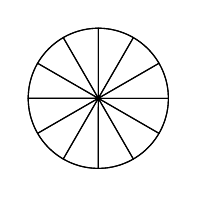
\begin{tikzpicture}[x=1.0cm,y=1.0cm, scale=0.5]
\draw (1.76,2.04) circle (1.78cm);
\draw [shift={(1.76,2.04)}]  (0,0) --  plot[domain=0.:0.5235987755982987,variable=\t]({1.*1.78*cos(\t r)+0.*1.78*sin(\t r)},{0.*1.78*cos(\t r)+1.*1.78*sin(\t r)}) -- cycle ;
\draw [shift={(1.76,2.04)}]  (0,0) --  plot[domain=0.5235987755982987:1.0471975511965974,variable=\t]({1.*1.78*cos(\t r)+0.*1.78*sin(\t r)},{0.*1.78*cos(\t r)+1.*1.78*sin(\t r)}) -- cycle ;
\draw [shift={(1.76,2.04)}]  (0,0) --  plot[domain=1.0471975511965974:1.5707963267948963,variable=\t]({1.*1.78*cos(\t r)+0.*1.78*sin(\t r)},{0.*1.78*cos(\t r)+1.*1.78*sin(\t r)}) -- cycle ;
\draw [shift={(1.76,2.04)}]  (0,0) --  plot[domain=1.5707963267948963:2.0943951023931953,variable=\t]({1.*1.78*cos(\t r)+0.*1.78*sin(\t r)},{0.*1.78*cos(\t r)+1.*1.78*sin(\t r)}) -- cycle ;
\draw [shift={(1.76,2.04)}]  (0,0) --  plot[domain=2.0943951023931953:2.617993877991494,variable=\t]({1.*1.78*cos(\t r)+0.*1.78*sin(\t r)},{0.*1.78*cos(\t r)+1.*1.78*sin(\t r)}) -- cycle ;
\draw [shift={(1.76,2.04)}]  (0,0) --  plot[domain=2.617993877991494:3.1415926535897927,variable=\t]({1.*1.78*cos(\t r)+0.*1.78*sin(\t r)},{0.*1.78*cos(\t r)+1.*1.78*sin(\t r)}) -- cycle ;
\draw [shift={(1.76,2.04)}]  (0,0) --  plot[domain=3.1415926535897927:3.6651914291880914,variable=\t]({1.*1.78*cos(\t r)+0.*1.78*sin(\t r)},{0.*1.78*cos(\t r)+1.*1.78*sin(\t r)}) -- cycle ;
\draw [shift={(1.76,2.04)}]  (0,0) --  plot[domain=3.6651914291880914:4.18879020478639,variable=\t]({1.*1.78*cos(\t r)+0.*1.78*sin(\t r)},{0.*1.78*cos(\t r)+1.*1.78*sin(\t r)}) -- cycle ;
\draw [shift={(1.76,2.04)}]  (0,0) --  plot[domain=4.18879020478639:4.712388980384689,variable=\t]({1.*1.78*cos(\t r)+0.*1.78*sin(\t r)},{0.*1.78*cos(\t r)+1.*1.78*sin(\t r)}) -- cycle ;
\draw [shift={(1.76,2.04)}]  (0,0) --  plot[domain=4.712388980384689:5.235987755982988,variable=\t]({1.*1.78*cos(\t r)+0.*1.78*sin(\t r)},{0.*1.78*cos(\t r)+1.*1.78*sin(\t r)}) -- cycle ;
\draw [shift={(1.76,2.04)}]  (0,0) --  plot[domain=5.235987755982988:5.759586531581286,variable=\t]({1.*1.78*cos(\t r)+0.*1.78*sin(\t r)},{0.*1.78*cos(\t r)+1.*1.78*sin(\t r)}) -- cycle ;
\draw [shift={(1.76,2.04)}]  (0,0) --  plot[domain=-0.5235987755983:0.,variable=\t]({1.*1.78*cos(\t r)+0.*1.78*sin(\t r)},{0.*1.78*cos(\t r)+1.*1.78*sin(\t r)}) -- cycle ;
\end{tikzpicture}}
  & \parbox[c][2cm]{0.13\textwidth}{\centering 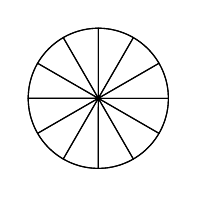
\begin{tikzpicture}[x=1.0cm,y=1.0cm, scale=0.5]
\draw (1.76,2.04) circle (1.78cm);
\draw [shift={(1.76,2.04)}]  (0,0) --  plot[domain=0.:0.5235987755982987,variable=\t]({1.*1.78*cos(\t r)+0.*1.78*sin(\t r)},{0.*1.78*cos(\t r)+1.*1.78*sin(\t r)}) -- cycle ;
\draw [shift={(1.76,2.04)}]  (0,0) --  plot[domain=0.5235987755982987:1.0471975511965974,variable=\t]({1.*1.78*cos(\t r)+0.*1.78*sin(\t r)},{0.*1.78*cos(\t r)+1.*1.78*sin(\t r)}) -- cycle ;
\draw [shift={(1.76,2.04)}]  (0,0) --  plot[domain=1.0471975511965974:1.5707963267948963,variable=\t]({1.*1.78*cos(\t r)+0.*1.78*sin(\t r)},{0.*1.78*cos(\t r)+1.*1.78*sin(\t r)}) -- cycle ;
\draw [shift={(1.76,2.04)}]  (0,0) --  plot[domain=1.5707963267948963:2.0943951023931953,variable=\t]({1.*1.78*cos(\t r)+0.*1.78*sin(\t r)},{0.*1.78*cos(\t r)+1.*1.78*sin(\t r)}) -- cycle ;
\draw [shift={(1.76,2.04)}]  (0,0) --  plot[domain=2.0943951023931953:2.617993877991494,variable=\t]({1.*1.78*cos(\t r)+0.*1.78*sin(\t r)},{0.*1.78*cos(\t r)+1.*1.78*sin(\t r)}) -- cycle ;
\draw [shift={(1.76,2.04)}]  (0,0) --  plot[domain=2.617993877991494:3.1415926535897927,variable=\t]({1.*1.78*cos(\t r)+0.*1.78*sin(\t r)},{0.*1.78*cos(\t r)+1.*1.78*sin(\t r)}) -- cycle ;
\draw [shift={(1.76,2.04)}]  (0,0) --  plot[domain=3.1415926535897927:3.6651914291880914,variable=\t]({1.*1.78*cos(\t r)+0.*1.78*sin(\t r)},{0.*1.78*cos(\t r)+1.*1.78*sin(\t r)}) -- cycle ;
\draw [shift={(1.76,2.04)}]  (0,0) --  plot[domain=3.6651914291880914:4.18879020478639,variable=\t]({1.*1.78*cos(\t r)+0.*1.78*sin(\t r)},{0.*1.78*cos(\t r)+1.*1.78*sin(\t r)}) -- cycle ;
\draw [shift={(1.76,2.04)}]  (0,0) --  plot[domain=4.18879020478639:4.712388980384689,variable=\t]({1.*1.78*cos(\t r)+0.*1.78*sin(\t r)},{0.*1.78*cos(\t r)+1.*1.78*sin(\t r)}) -- cycle ;
\draw [shift={(1.76,2.04)}]  (0,0) --  plot[domain=4.712388980384689:5.235987755982988,variable=\t]({1.*1.78*cos(\t r)+0.*1.78*sin(\t r)},{0.*1.78*cos(\t r)+1.*1.78*sin(\t r)}) -- cycle ;
\draw [shift={(1.76,2.04)}]  (0,0) --  plot[domain=5.235987755982988:5.759586531581286,variable=\t]({1.*1.78*cos(\t r)+0.*1.78*sin(\t r)},{0.*1.78*cos(\t r)+1.*1.78*sin(\t r)}) -- cycle ;
\draw [shift={(1.76,2.04)}]  (0,0) --  plot[domain=-0.5235987755983:0.,variable=\t]({1.*1.78*cos(\t r)+0.*1.78*sin(\t r)},{0.*1.78*cos(\t r)+1.*1.78*sin(\t r)}) -- cycle ;
\end{tikzpicture}}
   & \parbox[c][2cm]{0.13\textwidth}{\centering 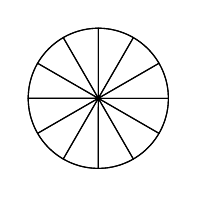
\begin{tikzpicture}[x=1.0cm,y=1.0cm, scale=0.5]
\draw (1.76,2.04) circle (1.78cm);
\draw [shift={(1.76,2.04)}]  (0,0) --  plot[domain=0.:0.5235987755982987,variable=\t]({1.*1.78*cos(\t r)+0.*1.78*sin(\t r)},{0.*1.78*cos(\t r)+1.*1.78*sin(\t r)}) -- cycle ;
\draw [shift={(1.76,2.04)}]  (0,0) --  plot[domain=0.5235987755982987:1.0471975511965974,variable=\t]({1.*1.78*cos(\t r)+0.*1.78*sin(\t r)},{0.*1.78*cos(\t r)+1.*1.78*sin(\t r)}) -- cycle ;
\draw [shift={(1.76,2.04)}]  (0,0) --  plot[domain=1.0471975511965974:1.5707963267948963,variable=\t]({1.*1.78*cos(\t r)+0.*1.78*sin(\t r)},{0.*1.78*cos(\t r)+1.*1.78*sin(\t r)}) -- cycle ;
\draw [shift={(1.76,2.04)}]  (0,0) --  plot[domain=1.5707963267948963:2.0943951023931953,variable=\t]({1.*1.78*cos(\t r)+0.*1.78*sin(\t r)},{0.*1.78*cos(\t r)+1.*1.78*sin(\t r)}) -- cycle ;
\draw [shift={(1.76,2.04)}]  (0,0) --  plot[domain=2.0943951023931953:2.617993877991494,variable=\t]({1.*1.78*cos(\t r)+0.*1.78*sin(\t r)},{0.*1.78*cos(\t r)+1.*1.78*sin(\t r)}) -- cycle ;
\draw [shift={(1.76,2.04)}]  (0,0) --  plot[domain=2.617993877991494:3.1415926535897927,variable=\t]({1.*1.78*cos(\t r)+0.*1.78*sin(\t r)},{0.*1.78*cos(\t r)+1.*1.78*sin(\t r)}) -- cycle ;
\draw [shift={(1.76,2.04)}]  (0,0) --  plot[domain=3.1415926535897927:3.6651914291880914,variable=\t]({1.*1.78*cos(\t r)+0.*1.78*sin(\t r)},{0.*1.78*cos(\t r)+1.*1.78*sin(\t r)}) -- cycle ;
\draw [shift={(1.76,2.04)}]  (0,0) --  plot[domain=3.6651914291880914:4.18879020478639,variable=\t]({1.*1.78*cos(\t r)+0.*1.78*sin(\t r)},{0.*1.78*cos(\t r)+1.*1.78*sin(\t r)}) -- cycle ;
\draw [shift={(1.76,2.04)}]  (0,0) --  plot[domain=4.18879020478639:4.712388980384689,variable=\t]({1.*1.78*cos(\t r)+0.*1.78*sin(\t r)},{0.*1.78*cos(\t r)+1.*1.78*sin(\t r)}) -- cycle ;
\draw [shift={(1.76,2.04)}]  (0,0) --  plot[domain=4.712388980384689:5.235987755982988,variable=\t]({1.*1.78*cos(\t r)+0.*1.78*sin(\t r)},{0.*1.78*cos(\t r)+1.*1.78*sin(\t r)}) -- cycle ;
\draw [shift={(1.76,2.04)}]  (0,0) --  plot[domain=5.235987755982988:5.759586531581286,variable=\t]({1.*1.78*cos(\t r)+0.*1.78*sin(\t r)},{0.*1.78*cos(\t r)+1.*1.78*sin(\t r)}) -- cycle ;
\draw [shift={(1.76,2.04)}]  (0,0) --  plot[domain=-0.5235987755983:0.,variable=\t]({1.*1.78*cos(\t r)+0.*1.78*sin(\t r)},{0.*1.78*cos(\t r)+1.*1.78*sin(\t r)}) -- cycle ;
\end{tikzpicture}}
  & \parbox[c][2cm]{0.13\textwidth}{\centering 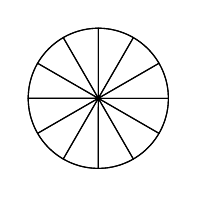
\begin{tikzpicture}[x=1.0cm,y=1.0cm, scale=0.5]
\draw (1.76,2.04) circle (1.78cm);
\draw [shift={(1.76,2.04)}]  (0,0) --  plot[domain=0.:0.5235987755982987,variable=\t]({1.*1.78*cos(\t r)+0.*1.78*sin(\t r)},{0.*1.78*cos(\t r)+1.*1.78*sin(\t r)}) -- cycle ;
\draw [shift={(1.76,2.04)}]  (0,0) --  plot[domain=0.5235987755982987:1.0471975511965974,variable=\t]({1.*1.78*cos(\t r)+0.*1.78*sin(\t r)},{0.*1.78*cos(\t r)+1.*1.78*sin(\t r)}) -- cycle ;
\draw [shift={(1.76,2.04)}]  (0,0) --  plot[domain=1.0471975511965974:1.5707963267948963,variable=\t]({1.*1.78*cos(\t r)+0.*1.78*sin(\t r)},{0.*1.78*cos(\t r)+1.*1.78*sin(\t r)}) -- cycle ;
\draw [shift={(1.76,2.04)}]  (0,0) --  plot[domain=1.5707963267948963:2.0943951023931953,variable=\t]({1.*1.78*cos(\t r)+0.*1.78*sin(\t r)},{0.*1.78*cos(\t r)+1.*1.78*sin(\t r)}) -- cycle ;
\draw [shift={(1.76,2.04)}]  (0,0) --  plot[domain=2.0943951023931953:2.617993877991494,variable=\t]({1.*1.78*cos(\t r)+0.*1.78*sin(\t r)},{0.*1.78*cos(\t r)+1.*1.78*sin(\t r)}) -- cycle ;
\draw [shift={(1.76,2.04)}]  (0,0) --  plot[domain=2.617993877991494:3.1415926535897927,variable=\t]({1.*1.78*cos(\t r)+0.*1.78*sin(\t r)},{0.*1.78*cos(\t r)+1.*1.78*sin(\t r)}) -- cycle ;
\draw [shift={(1.76,2.04)}]  (0,0) --  plot[domain=3.1415926535897927:3.6651914291880914,variable=\t]({1.*1.78*cos(\t r)+0.*1.78*sin(\t r)},{0.*1.78*cos(\t r)+1.*1.78*sin(\t r)}) -- cycle ;
\draw [shift={(1.76,2.04)}]  (0,0) --  plot[domain=3.6651914291880914:4.18879020478639,variable=\t]({1.*1.78*cos(\t r)+0.*1.78*sin(\t r)},{0.*1.78*cos(\t r)+1.*1.78*sin(\t r)}) -- cycle ;
\draw [shift={(1.76,2.04)}]  (0,0) --  plot[domain=4.18879020478639:4.712388980384689,variable=\t]({1.*1.78*cos(\t r)+0.*1.78*sin(\t r)},{0.*1.78*cos(\t r)+1.*1.78*sin(\t r)}) -- cycle ;
\draw [shift={(1.76,2.04)}]  (0,0) --  plot[domain=4.712388980384689:5.235987755982988,variable=\t]({1.*1.78*cos(\t r)+0.*1.78*sin(\t r)},{0.*1.78*cos(\t r)+1.*1.78*sin(\t r)}) -- cycle ;
\draw [shift={(1.76,2.04)}]  (0,0) --  plot[domain=5.235987755982988:5.759586531581286,variable=\t]({1.*1.78*cos(\t r)+0.*1.78*sin(\t r)},{0.*1.78*cos(\t r)+1.*1.78*sin(\t r)}) -- cycle ;
\draw [shift={(1.76,2.04)}]  (0,0) --  plot[domain=-0.5235987755983:0.,variable=\t]({1.*1.78*cos(\t r)+0.*1.78*sin(\t r)},{0.*1.78*cos(\t r)+1.*1.78*sin(\t r)}) -- cycle ;
\end{tikzpicture}}
  \\
    \hline
     Escreva, por extenso, a fração de pizza consumida por cada pessoa&                                        &                                        &                                         &                                        \\
    \hline
     Escreva, usando símbolos matemáticos, a fração de pizza consumida por cada pessoa &                                        &                                        &                                         &                                        \\
    \hline
  \end{tabular}
\end{center}

\begin{enumerate} [label=\alph*)] %d
  \item Na sua opinião, qual maneira de representar fração ``gasta menos lápis'': pintando, escrevendo por extenso ou usando simbolos matemáticos?
  \item Na sua opinião, qual a representação que mais rapidamente ajuda a decidir quem comeu mais e quem comeu menos pizza?
\end{enumerate} %d

\ifdefined\prof

\begin{solucao}

\begin{center}
\addtolength{\cellspacetoplimit}{1.5pt}
\addtolength{\cellspacebottomlimit}{1.5pt}
% \renewcommand{\arraystretch}{1.5}
  \begin{tabular}{|>{\centering}S{m{0.13\textwidth}}|>{\centering}S{m{0.13\textwidth}}|>{\centering}S{m{0.13\textwidth}}|>{\centering}S{m{0.13\textwidth}}|}
\hline
         Pedro &  Isabella  &    Bernardo  &   Manuela  \tabularnewline
      \hline
       \begin{tikzpicture}[x=1mm,y=1mm, scale=.7]
        \draw[fill=common, fill opacity=.3] (0,0) circle (10);
        \fill[attention] (90:10) arc (90:210:10) -- (0,0) -- cycle;
        \foreach \x in {0,30,...,150}\draw (\x:10) -- (\x:-10);
       \end{tikzpicture}&
       \begin{tikzpicture}[x=1mm,y=1mm, scale=.7]
        \draw[fill=common, fill opacity=.3] (0,0) circle (10);
        \fill[attention] (210:10) arc (210:360:10) -- (0,0) -- cycle;
        \foreach \x in {0,30,...,150}\draw (\x:10) -- (\x:-10);
       \end{tikzpicture}&
       \begin{tikzpicture}[x=1mm,y=1mm, scale=.7]
        \draw[fill=common, fill opacity=.3] (0,0) circle (10);
        \fill[attention] (0:10) arc (0:60:10) -- (0,0) -- cycle;
        \foreach \x in {0,30,...,150}\draw (\x:10) -- (\x:-10);
       \end{tikzpicture}&
       \begin{tikzpicture}[x=1mm,y=1mm, scale=.7]
        \draw[fill=common, fill opacity=.3] (0,0) circle (10);
        \fill[attention] (60:10) arc (60:90:10) -- (0,0) -- cycle;
        \foreach \x in {0,30,...,150}\draw (\x:10) -- (\x:-10);
       \end{tikzpicture}\tabularnewline
      \hline
      \centering  { quatro doze avos}  & \centering  { cinco doze avos}  & \centering  { dois doze avos}  & {\centering  { um doze avos}}   \tabularnewline
      \hline
       \setlength\extrarowheight{10pt}\centering $\displaystyle\frac{4}{12}$& \centering  $\displaystyle\frac{5}{12}$& \centering  $\displaystyle\frac{2}{12}$ & \centering  $\displaystyle\frac{1}{12}$ \tabularnewline
       \hline
    \end{tabular}
\end{center}
\begin{enumerate} [label=\alph*)] %s
    \item       A que usa a notação simbólica matemática.
    \item       As respostas podem variar de pessoa para pessoa. No entanto, a justificativa deve ser coerente com a resposta. Discuta com a turma as diferentes respostas.
\end{enumerate} %s

\end{solucao}
\fi

\end{document}